\documentclass[lang=cn]{elegantpaper}
\author{Jiang Zifeng\\522030910097}
\usepackage{hyperref}
\date{}
\title{Project 1 Dimensionality Reduction\footnote{Code is in my \href{https://github.com/Angzif/CS3319-PROJECT1}{Github repository}}}

\begin{document}
\maketitle

\section{Data Preprocess}

\subsection{Overview}
The dataset used in this study is the Animals with Attributes 2 (AwA2) dataset, which contains 37,322 images of 50 animal classes. The deep learning features were pre-extracted and split into training \(60\%\) and testing \(40\%\) sets. The data preprocessing steps include normalization and standardization to ensure consistent feature scales.

\subsection{Code Implementation}

\begin{lstlisting}[language=Python]
def load_data(feature_path, label_path):
    """
    Load featrues and labels
    :param feature_path: Features file path
    :param label_path: Label file path
    :return: features (numpy), labels (numpy)
    """
    features = np.loadtxt(feature_path)
    labels = np.loadtxt(label_path)
    return features, labels


def split_data(features, labels, test_ratio=0.4, random_state=42):
    """
    split train dataset and test dataset
    :param features: Features
    :param labels: Labels
    :param test_ratio: The ratio of test dataset
    :param random_state: Random seed
    :return: train_features, test_features, train_labels, test_labels
    """
    np.random.seed(random_state)
    shuffle_index = np.random.permutation(len(labels))
    shuffled_features = features[shuffle_index]
    shuffled_labels = labels[shuffle_index]

    test_size = int(len(labels) * test_ratio)
    train_features = shuffled_features[:-test_size]
    test_features = shuffled_features[-test_size:]
    train_labels = shuffled_labels[:-test_size]
    test_labels = shuffled_labels[-test_size:]

    return train_features, test_features, train_labels, test_labels


def normalize_data(data):
    """
    normalize data with mean 0 and std 1
    :param data: input data (numpy)
    :return: normalized data
    """
    mean = np.mean(data, axis=0)
    std = np.std(data, axis=0)
    normalized_data = (data - mean) / std
    return normalized_data


def scale_data(data, x_min=0, x_max=1):
    """
    scale data:scale data to range [x_min, x_max]
    :param data: input data (numpy)
    :param x_min: minmum data
    :param x_max: maximum data
    :return: scaled data
    """
    min_val = np.min(data, axis=0)
    max_val = np.max(data, axis=0)
    scaled_data = (data - min_val) / (max_val - min_val) * (x_max - x_min) + x_min
    return scaled_data


def save_data(data, save_path):
    """
    save data
    :param data: data to be saved (numpy)
    :param save_path: save path
    """
    np.savetxt(save_path, data)


def data_preprocess(feature_path, label_path, output_dir, test_ratio=0.4, normalize=True, scale=False):
    """
    main function of data preprocess
    :param feature_path: feature file path
    :param label_path: label file path
    :param output_dir: output dirctory
    :param test_ratio: the ratio of test data
    :param normalize: normalization(True or False)
    :param scale: scale(True or False)
    """
    # Load data
    features, labels = load_data(feature_path, label_path)
    print(f"Loaded {len(features)} samples with {features.shape[1]} features.")

    # Split dataset to traning set and testing set
    train_features, test_features, train_labels, test_labels = split_data(features, labels, test_ratio)
    print(f"Training set size: {len(train_features)}")
    print(f"Testing set size: {len(test_features)}")

    # Normalization or scale
    if normalize:
        train_features = normalize_data(train_features)
        test_features = normalize_data(test_features)
        print("Data normalized (mean=0, std=1).")
    elif scale:
        train_features = scale_data(train_features)
        test_features = scale_data(test_features)
        print(f"Data scaled to [0, 1].")

    # Create output directory
    os.makedirs(output_dir, exist_ok=True)

    # save data
    save_data(train_features, os.path.join(output_dir, "train_features.txt"))
    save_data(test_features, os.path.join(output_dir, "test_features.txt"))
    save_data(train_labels, os.path.join(output_dir, "train_labels.txt"))
    save_data(test_labels, os.path.join(output_dir, "test_labels.txt"))
    print(f"Processed data saved to {output_dir}.")
\end{lstlisting}

\section{Find The Best Byperparameter of SVM}

\subsection{Overview}

To determine the value of C in SVM, we can use a grid search with cross-validation. Here is an example code snippet to perform this task:

\subsection{Code Implement}

\begin{lstlisting}[language=Python]
def find_bestC(train_feature, train_label):
    """
    Determine the best value of C in SVM by GridSearchCV 
    :param train_feature: Features
    :param train_label: Labels
    :return: The value of C
    """
    param_grid = [
        {'C': [0.000001, 0.00001, 0.0001, 0.001, 0.01, 0.1, 1, 10, 100], 
         'kernel': ['linear'], 
         'decision_function_shape': ['ovr']},
    ]

    svc = SVC()
    grid_search = GridSearchCV(svc, param_grid, cv=5, verbose=3, n_jobs=4)
    grid_search.fit(train_feature, train_label)

    print("Best parameters: ", grid_search.best_params_)
    print("Best cross-validation score: ", grid_search.best_score_)
    return grid_search.best_params_['C']
\end{lstlisting}

\subsection{Output}

The results of the code are as follows:

\begin{lstlisting}
    Loading labels from: dataset/processed_data\train_labels.txt
    Loading features from: dataset/processed_data\train_features.txt
    Fitting 5 folds for each of 9 candidates, totalling 45 fits
    [CV 1/5] END C=1e-06, decision_function_shape=ovr, kernel=linear;, score=0.045 total time=19.7min
    [CV 2/5] END C=1e-06, decision_function_shape=ovr, kernel=linear;, score=0.045 total time=20.1min
    [CV 3/5] END C=1e-06, decision_function_shape=ovr, kernel=linear;, score=0.044 total time=20.2min
    [CV 4/5] END C=1e-06, decision_function_shape=ovr, kernel=linear;, score=0.044 total time=20.3min
    [CV 1/5] END C=1e-05, decision_function_shape=ovr, kernel=linear;, score=0.782 total time=14.1min
    [CV 2/5] END C=1e-05, decision_function_shape=ovr, kernel=linear;, score=0.786 total time=14.2min
    [CV 3/5] END C=1e-05, decision_function_shape=ovr, kernel=linear;, score=0.788 total time=14.2min
    ...
    [CV 1/5] END C=100, decision_function_shape=ovr, kernel=linear;, score=0.915 total time= 3.3min
    [CV 2/5] END C=100, decision_function_shape=ovr, kernel=linear;, score=0.927 total time= 3.3min
    [CV 3/5] END C=100, decision_function_shape=ovr, kernel=linear;, score=0.928 total time= 3.0min
    [CV 5/5] END C=100, decision_function_shape=ovr, kernel=linear;, score=0.915 total time= 2.1min
    [CV 4/5] END C=100, decision_function_shape=ovr, kernel=linear;, score=0.924 total time= 2.2min
    Best parameters:  {'C': 0.001, 'decision_function_shape': 'ovr', 'kernel': 'linear'}
    Best cross-validation score:  0.928239550934982
    Best C parameter: 0.001
\end{lstlisting}

The result indicates that the best parameters for the SVM model are $C = 0.001$, with a decision function shape of 'ovr' (one-vs-rest) and a kernel type of 'linear'. The cross-validation score achieved is approximately 0.928, which indicates that the model has a high level of accuracy in predicting the outcomes across different folds.

\section{SVM classification}

\subsection{Overview}

After determining the value of C, we can proceed with applying this parameter to our SVM classifier for the final model training and evaluation on the test set. The goal is to assess how well the SVM performs when using the optimal parameters found through cross-validation.

\subsection{Code Implementation}

\begin{lstlisting}[language=Python]
def svm_classifier(train_features, train_labels, test_features, test_labels, C=1e-3, k_fold=5):
    """
    Use linear SVM for classification
    :param train_features: Train Features`'
    :param train_labels: Train Labels
    :param test_features: Test Features`'
    :param test_labels: Test Lables
    :param C: C in SVM
    :param k_fold
    :return: The accuracy on test set
    """
    # Linear SVM initialization
    svm = SVC(kernel='linear', C=C)

    # K fold
    kf = KFold(n_splits=k_fold, shuffle=True, random_state=42)
    cv_scores = cross_val_score(svm, train_features, train_labels, cv=kf, scoring='accuracy')
    print(f"Cross-validation accuracy: {np.mean(cv_scores):.4f} (±{np.std(cv_scores):.4f})")

    # training
    svm.fit(train_features, train_labels)

    # prediction
    test_predictions = svm.predict(test_features)
    test_accuracy = accuracy_score(test_labels, test_predictions)
    print(f"Test accuracy: {test_accuracy:.4f}")

    # output report
    print("Classification Report:")
    print(classification_report(test_labels, test_predictions))

    return test_accuracy
\end{lstlisting}

\subsection{Output}

The results of SVM cliassification are as follows:

\begin{lstlisting}
    Cross-validation accuracy: 0.9294 (±0.0043)
    Test accuracy: 0.9307
    Classification Report:
                  precision    recall  f1-score   support
    
             1.0       0.94      0.88      0.91       438
             2.0       0.93      0.96      0.95       341
             3.0       0.87      0.87      0.87       112
             4.0       0.79      0.80      0.79        84
             5.0       0.98      0.98      0.98       230
             6.0       0.92      0.91      0.91       301
             7.0       0.92      0.95      0.94       648
             8.0       0.89      0.91      0.90       411
             9.0       0.75      0.36      0.49        66
            10.0       0.86      0.86      0.86       202
            11.0       0.99      0.95      0.97        78
            12.0       0.97      0.91      0.94        34
            13.0       0.99      1.00      0.99       334
            14.0       0.93      0.95      0.94       300
            15.0       0.99      1.00      0.99       299
...
            43.0       0.99      0.98      0.99       411
            44.0       0.57      0.47      0.51        81
            45.0       0.99      0.99      0.99       331
            46.0       0.93      0.91      0.92       433
            47.0       0.92      0.70      0.79        83
            48.0       0.89      0.90      0.89       203
            49.0       0.86      0.88      0.87       515
            50.0       0.93      0.94      0.94       365
    
        accuracy                           0.93     14928
       macro avg       0.91      0.90      0.90     14928
    weighted avg       0.93      0.93      0.93     14928
\end{lstlisting}

\section{Reduction}

\subsection{Overview}

To reduction, we can use PCA, Autoencoder and LLE methods to reduce the dimensionality of the data. We will compare the performance of these methods with SVM classifier. The goal is to find out which method can best represent the original dataset while maintaining a high level of accuracy.

\subsection{Code Implementation}

\begin{lstlisting}[language=Python]
def benchmark():
    """
    Benchmark: Use original data
    """
    svm = SVC(kernel='linear', random_state=random_state)
    svm.fit(train_feature, train_label)
    train_score = svm.score(train_feature, train_label)
    test_score = svm.score(test_feature, test_label)
    print(f"原始特征的性能 - 训练集准确率: {train_score:.4f}, 测试集准确率: {test_score:.4f}")
    return train_score, test_score

def genetic_reduction(n_components, population_size=20, num_generations=10):
    """
    Genetic algorithm
    :param n_components: target dim
    :param population_size: population size
    :param num_generations: number of generation
    :return: selected features
    """
    print(f"使用遗传算法选择 {n_components} 个特征...")

    # Initialization
    num_features = train_feature.shape[1]
    population = [np.random.choice([0, 1], size=num_features, p=[0.5, 0.5]) for _ in range(population_size)]

    def fitness(individual):
        """
        Fitness function: use SVM 
        :param individual: individual)
        :return: score
        """
        selected_features = individual == 1
        if np.sum(selected_features) == 0:  # 如果没有选择任何特征,适应度为 0
            return 0
        X_train_selected = train_feature[:, selected_features]
        X_test_selected = test_feature[:, selected_features]
        svm = SVC(kernel='linear', random_state=random_state)
        svm.fit(X_train_selected, train_label)
        return svm.score(X_test_selected, test_label)

    for generation in range(num_generations):
        print(f"Generation {generation + 1}/{num_generations}")

        # calculate fitness
        fitness_scores = [fitness(individual) for individual in population]

        # selection
        fitness_scores = np.array(fitness_scores)
        fitness_scores = fitness_scores / np.sum(fitness_scores)  # 归一化
        selected_indices = np.random.choice(range(population_size), size=population_size, p=fitness_scores)
        selected_population = [population[i] for i in selected_indices]

        new_population = []
        for i in range(0, population_size, 2):
            parent1 = selected_population[i]
            parent2 = selected_population[i + 1] if i + 1 < population_size else selected_population[0]
            crossover_point = random.randint(1, num_features - 1)
            child1 = np.concatenate([parent1[:crossover_point], parent2[crossover_point:]])
            child2 = np.concatenate([parent2[:crossover_point], parent1[crossover_point:]])
            new_population.extend([child1, child2])

        for individual in new_population:
            if random.random() < 0.1:  # 变异概率
                mutation_point = random.randint(0, num_features - 1)
                individual[mutation_point] = 1 - individual[mutation_point]

        population = new_population

    # select best individual
    best_individual = max(population, key=fitness)
    selected_features = best_individual == 1
    print("遗传算法特征选择完成!")
    return selected_features
def evaluate_genetic_reduction(n_components):
    """
    evaluate genetic algorithm
    :param n_components: target dim
    :return: accuracy of train and test set, tiem cost
    """
    start_time = time.time()
    selected_features = genetic_reduction(n_components)
    train_F = train_feature[:, selected_features]
    test_F = test_feature[:, selected_features]
    end_time = time.time()


    svm = SVC(kernel='linear', random_state=random_state)
    svm.fit(train_F, train_label)
    train_score = svm.score(train_F, train_label)
    test_score = svm.score(test_F, test_label)
    print(f"遗传算法降维到 {n_components} 个特征 - 训练集准确率: {train_score:.4f}, 测试集准确率: {test_score:.4f}")
    return train_score, test_score, end_time - start_time

def pca_reduction(n_components):
    """
    PCA 
    :param n_components: target dim
    :return: train features, train labels, cost time
    """
    print(f"使用 PCA 降维到 {n_components} 维...")
    start_time = time.time()
    pca = PCA(n_components=n_components, random_state=random_state)
    train_F = pca.fit_transform(train_feature)
    test_F = pca.transform(test_feature)
    end_time = time.time()
    print(f"PCA 降维完成!耗时: {end_time - start_time:.2f} 秒")
    return train_F, test_F, end_time - start_time

def tsne_reduction(n_components):
    """
    t-SNE
    :param n_components: target dim
    :return: train features, train labels, cost time
    """
    print(f"使用 t-SNE 降维到 {n_components} 维...")
    start_time = time.time()
    tsne = TSNE(n_components=n_components, method='exact', random_state=random_state)
    train_F = tsne.fit_transform(train_feature)
    test_F = tsne.fit_transform(test_feature)
    end_time = time.time()
    print(f"t-SNE 降维完成!耗时: {end_time - start_time:.2f} 秒")
    return train_F, test_F, end_time - start_time

def lle_reduction(n_components):
    """
    LLE
    :param n_components: target dim
    :return: train features, train labels, cost time
    """
    print(f"使用 LLE 降维到 {n_components} 维...")
    start_time = time.time()
    lle = LocallyLinearEmbedding(n_components=n_components, random_state=random_state)
    train_F = lle.fit_transform(train_feature)
    test_F = lle.fit_transform(test_feature)
    end_time = time.time()
    print(f"LLE 降维完成!耗时: {end_time - start_time:.2f} 秒")
    return train_F, test_F, end_time - start_time

def autoencoder_reduction(n_components):
    """
    AutoEncoder
    :param n_components: target dim
    :return: train features, train labels, cost time
    """
    print(f"使用 AutoEncoder 降维到 {n_components} 维...")

    class Autoencoder(nn.Module):
        def __init__(self, input_dim, hidden_dim):
            super(Autoencoder, self).__init__()
            self.encoder = nn.Sequential(
                nn.Linear(input_dim, 128),
                nn.ReLU(),
                nn.Linear(128, hidden_dim),
                nn.ReLU()
            )
            self.decoder = nn.Sequential(
                nn.Linear(hidden_dim, 128),
                nn.ReLU(),
                nn.Linear(128, input_dim),
                nn.Sigmoid()
            )
        
        def forward(self, x):
            encoded = self.encoder(x)
            decoded = self.decoder(encoded)
            return decoded

    device = torch.device("cuda" if torch.cuda.is_available() else "cpu")
    train_tensor = torch.tensor(train_feature, dtype=torch.float32).to(device)
    test_tensor = torch.tensor(test_feature, dtype=torch.float32).to(device)
    train_dataset = TensorDataset(train_tensor)
    train_loader = DataLoader(train_dataset, batch_size=64, shuffle=True)

    # 训练 AutoEncoder
    model = Autoencoder(input_dim=train_feature.shape[1], hidden_dim=n_components).to(device)
    criterion = nn.MSELoss()
    optimizer = optim.Adam(model.parameters(), lr=1E-4)

    start_time = time.time()
    epochs = 20
    for epoch in range(epochs):
        for data in train_loader:
            inputs = data[0]
            optimizer.zero_grad()
            outputs = model(inputs)
            loss = criterion(outputs, inputs)
            loss.backward()
            optimizer.step()
        print(f"Epoch {epoch+1}, Loss: {loss.item()}")

    # 降维
    train_F = model.encoder(train_tensor).cpu().detach().numpy()
    test_F = model.encoder(test_tensor).cpu().detach().numpy()
    end_time = time.time()
    print(f"AutoEncoder 降维完成!耗时: {end_time - start_time:.2f} 秒")
    return train_F, test_F, end_time - start_time
\end{lstlisting}

\subsection{Output}

The output of code above are as follows:
\begin{lstlisting}
    原始特征的性能 - 训练集准确率: 0.9994, 测试集准确率: 0.9253
    === 正在评估 PCA ===
    使用 PCA 降维到 512 维...
    PCA 降维完成!耗时: 5.85 秒
    PCA 降维到 512 维 - 训练集准确率: 0.9994, 测试集准确率: 0.9177
    使用 PCA 降维到 256 维...
    ...

    === 时间性能比较 ===
    GENETIC的时间性能: [419.27543234825134,287.1231644153595,218.4008662700653,149.43833923339844,152.6374523639679, 124.58902382850647]
    PCA 的时间性能: [5.85403299331665, 2.7441177368164062, 2.6120896339416504, 1.6897475719451904, 1.2859976291656494, 1.003394365310669]
    LLE 的时间性能: [964.5589406490326, 924.242021560669, 903.0546798706055, 901.4459507465363, 899.1392750740051, 916.3233752250671]
    AUTOENCODER 的时间性能: [9.29868459701538, 11.854812622070312, 10.281035900115967, 10.867778778076172, 10.260303020477295, 10.499478816986084]
\end{lstlisting}

\section{Summary}

The summary of the result are shown in figures\ref{TIME},\ref{TrainAccuracy},\ref{TestAccuracy}

\begin{figure}[h]
    \centering
    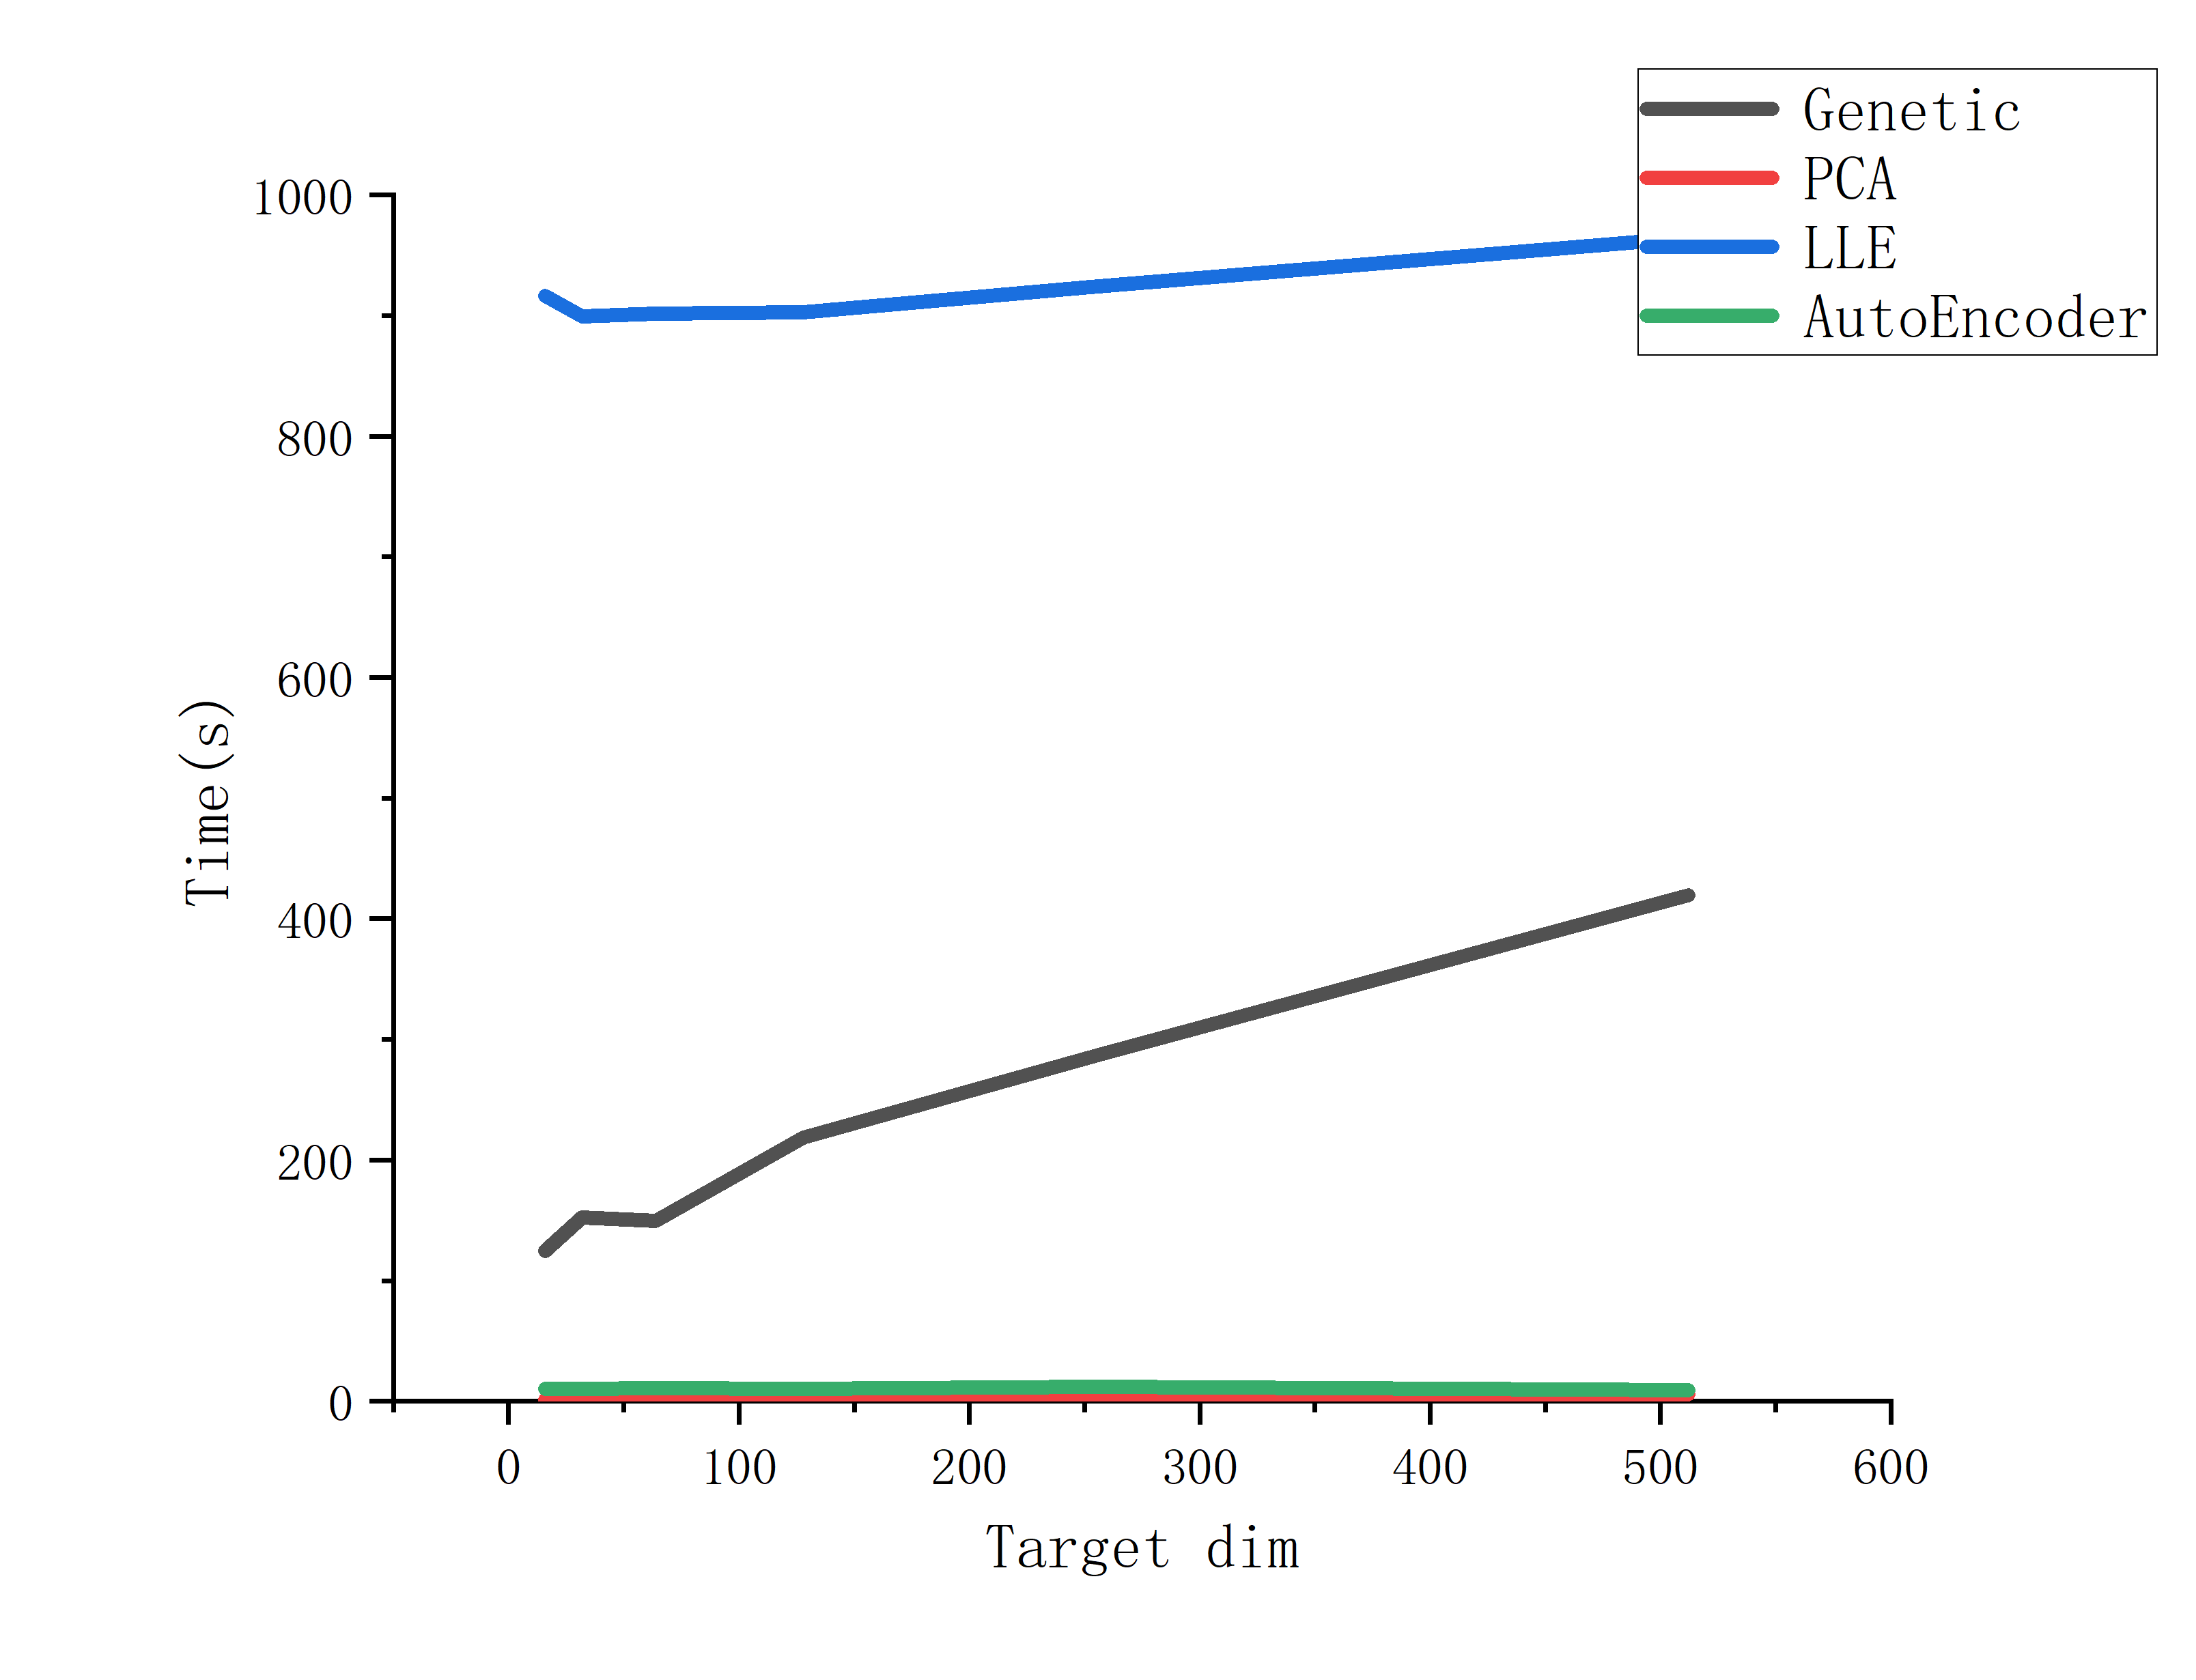
\includegraphics[width=0.7\textwidth]{TIME.png}
    \caption{Time}
    \label{TIME}
\end{figure}

\begin{figure}[h]
    \centering
    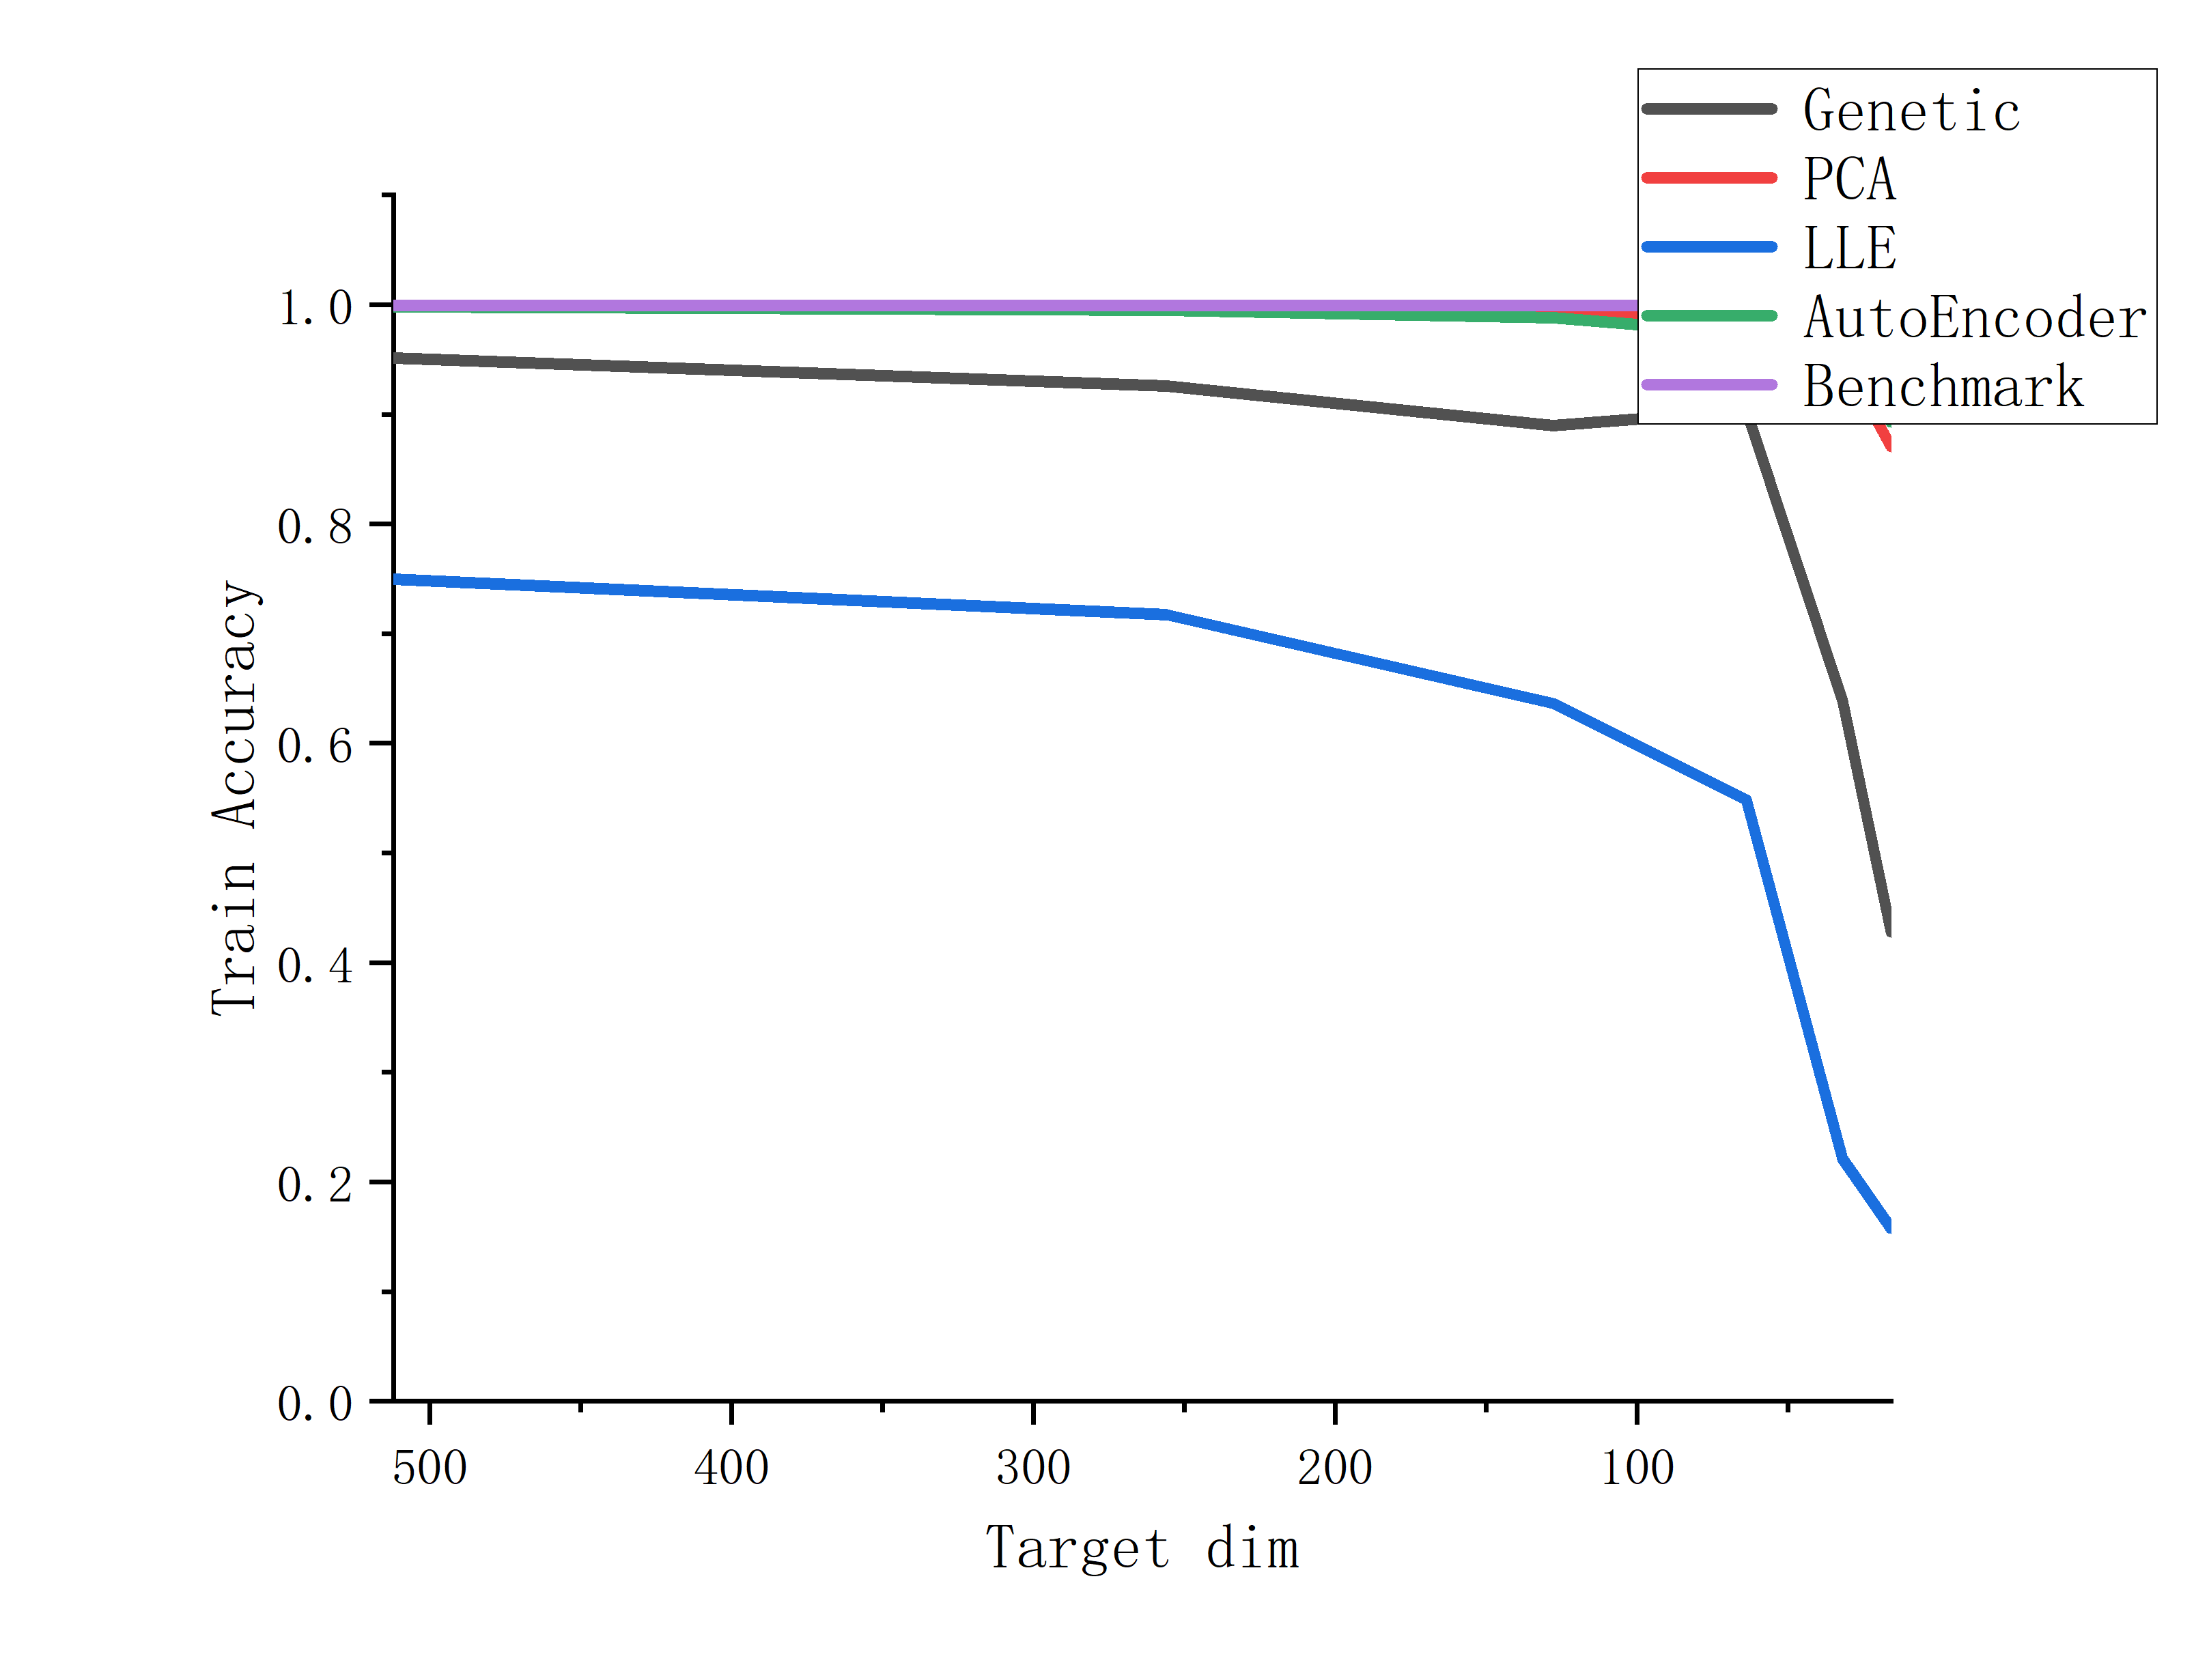
\includegraphics[width=0.7\textwidth]{TrainAccuracy.png}
    \caption{Train Accuracy}
    \label{TrainAccuracy}
\end{figure}

\begin{figure}[h]
    \centering
    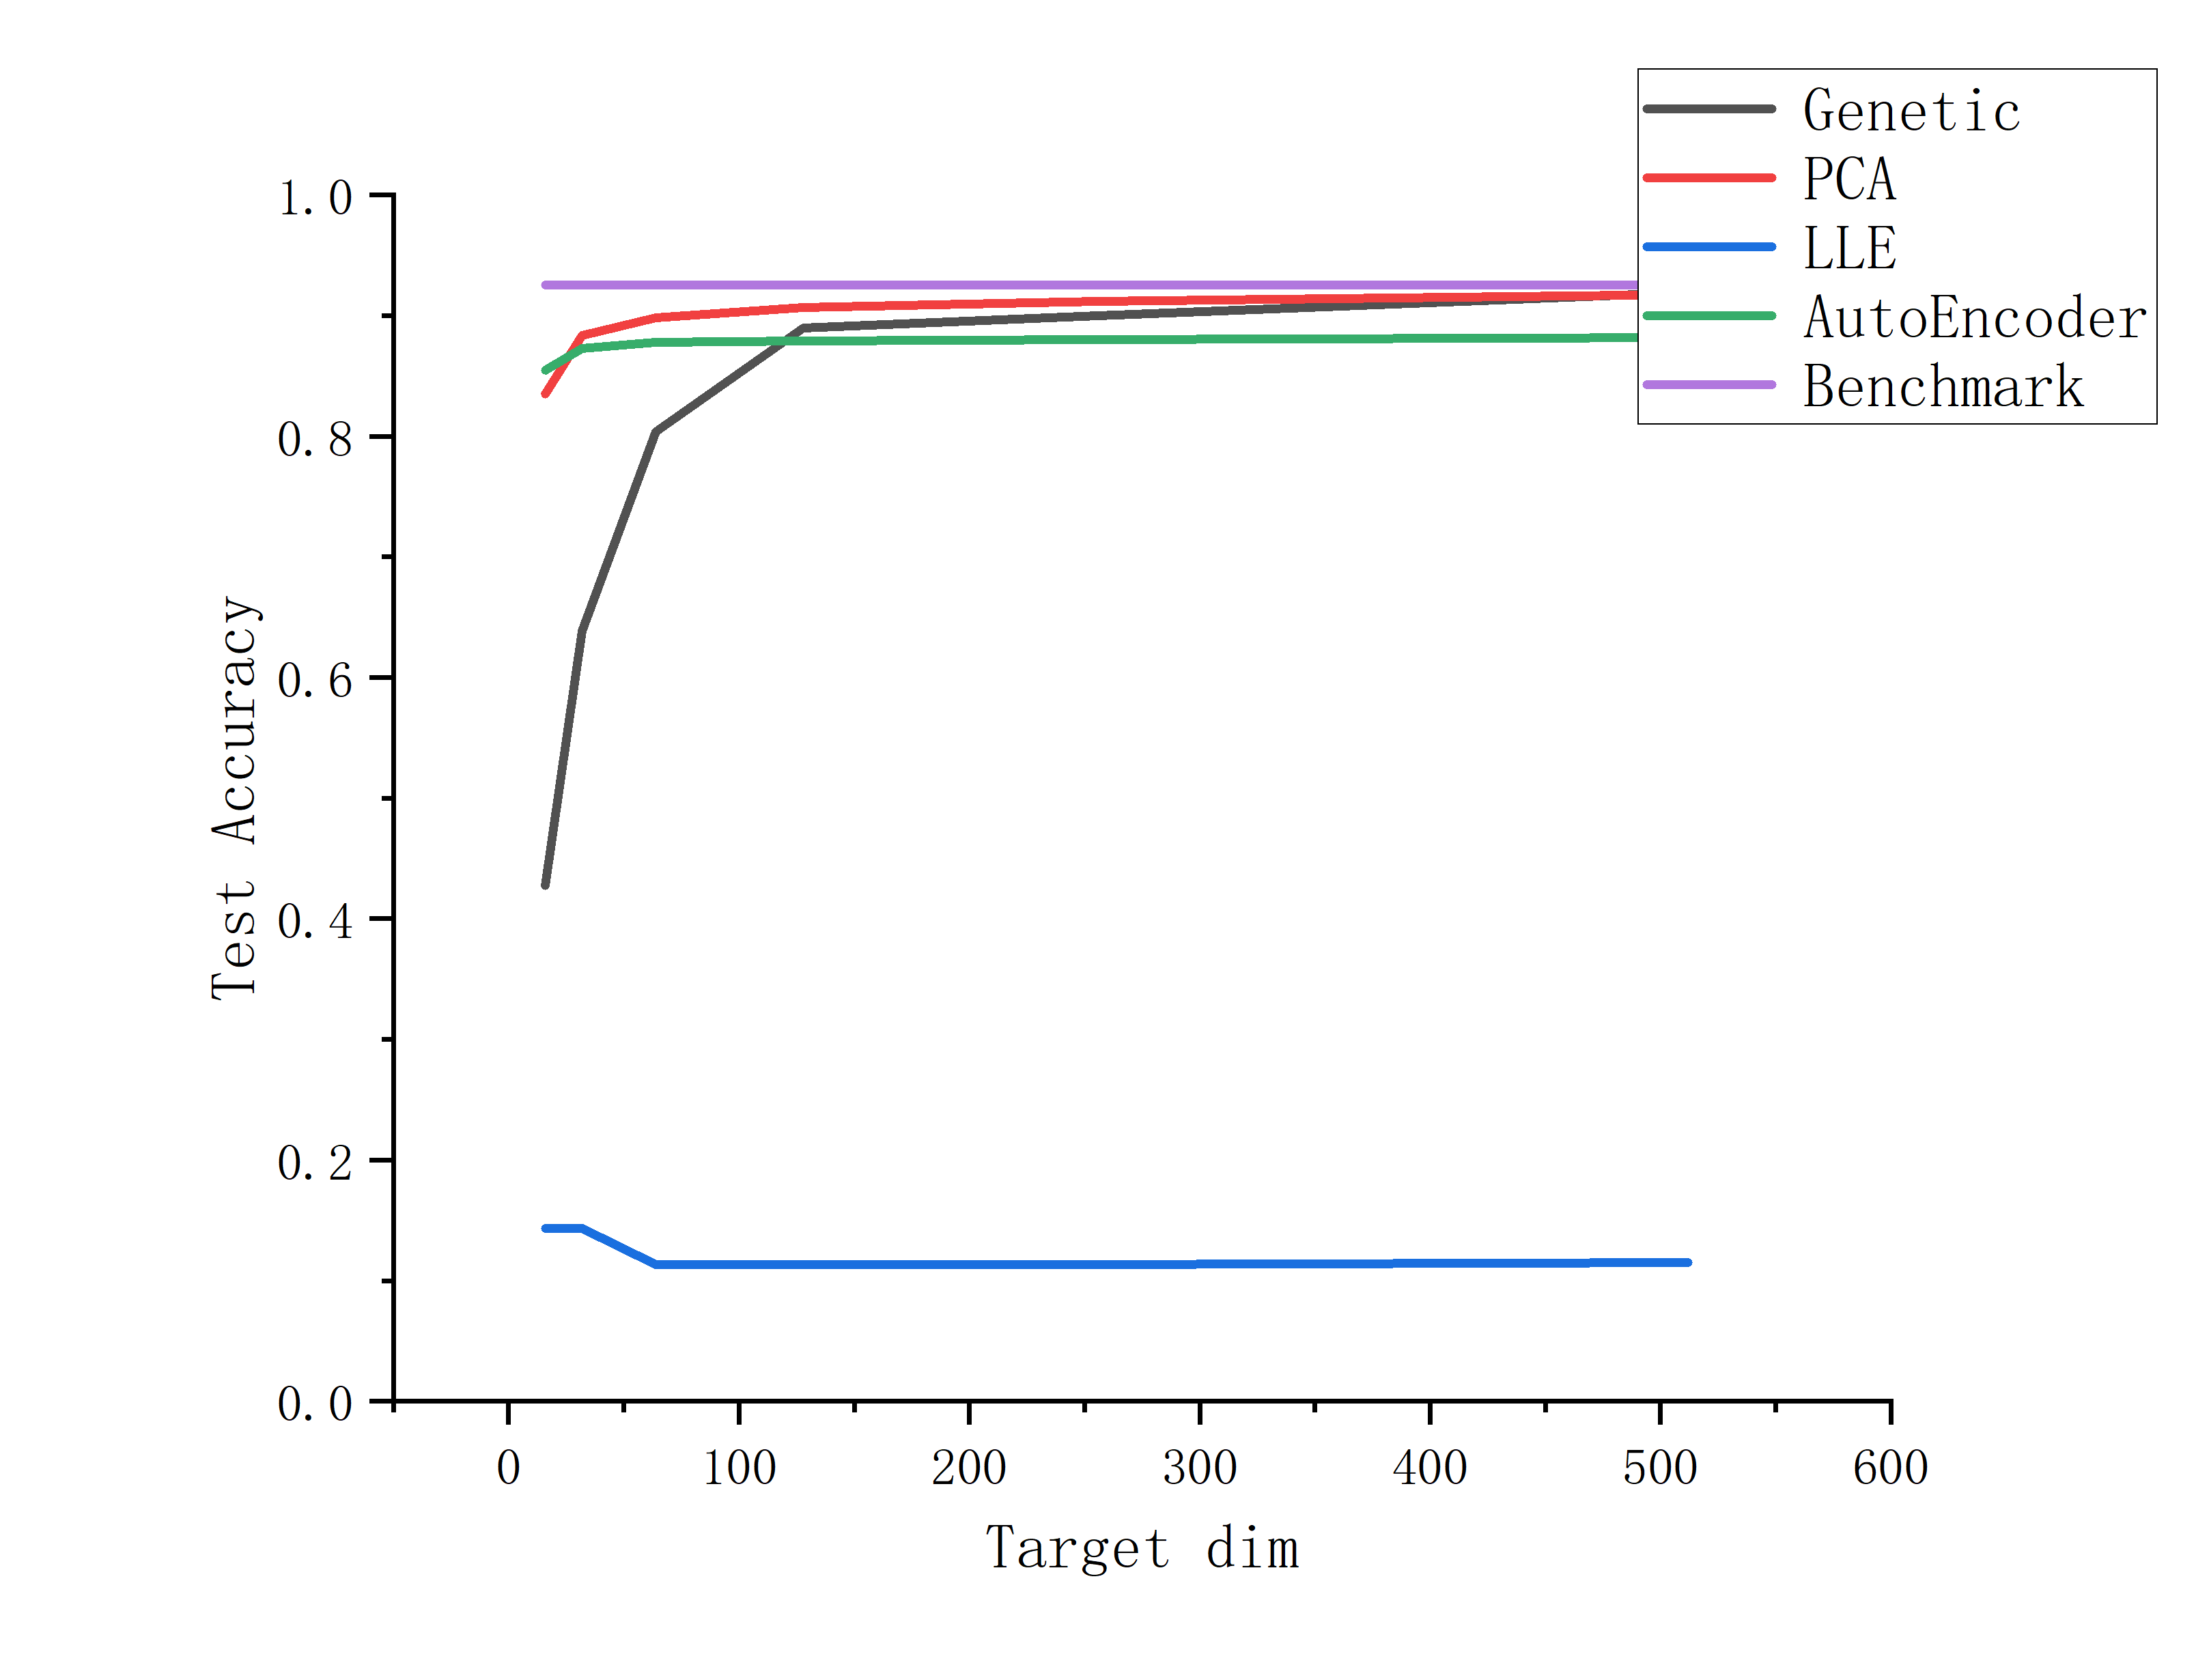
\includegraphics[width=0.7\textwidth]{TestAccuracy.png}
    \caption{Test Accuracy}
    \label{TestAccuracy}
\end{figure}

These figure indicates that PCA is the fastest algorithm among these algorithms. The accuracy of training set and test set are both high, which means our model has a good performance on this dataset.

The AutoEncoder has similar performance while the performance of LLE is not satisfactory
\end{document}